% DOC SETTINGS ===================================
\documentclass{article}
\usepackage[utf8]{inputenc}
\usepackage{steinmetz}
\usepackage{mathtools}  
\usepackage{multicol}
\usepackage{circuitikz}
\usepackage{listings}
\usepackage{geometry}
\usepackage{fancyhdr}
\usepackage{media9}
\pagestyle{fancy}
\lhead{ECE2714 Problem Set 5}
\rhead{Kavin Thirukonda 2021}
\fancyheadoffset{0mm}
 \geometry{
 a4paper,
 total={170mm,257mm},
 left=20mm,
 top=25mm,
 }
\mathtoolsset{showonlyrefs} 
\cfoot{}
% DOC SETTINGS ===================================
\begin{document}
\begin{enumerate}
    \item Consider the function x[n] given by
    \begin{equation}
        x[n] = \left(\frac{1}{4}\right)^{-n}u[-n-1],
    \end{equation}
    and impulse response h[n] given by
    \begin{equation}
        h[n] = u[n-1],
    \end{equation}
    Compute the convolution y[n] = x[n] * h[n].
    
    Hint: First perform the calculation for the case in which $n \geq 0$. Next, perform the convolution for the case in which $n < 0$.
    \begin{equation}
        y[t] = \sum_{k=-\infty}^{\infty} \left(\frac{1}{4}\right)^{-k}\underbrace{u[-k-1]}_{k>-1\Rightarrow0}\underbrace{u[n-k+1]}_{k>n+1\Rightarrow0}
    \end{equation}
    \begin{center}
        This summation can be broken up in to different summations that will allow us to perform the calculation more easily using what we know about the functions and where they are non-zero:
    \end{center}
    \begin{align}
        &y[t] = \sum_{k=-1}^{-\infty} \left(\frac{1}{4}\right)^{-k} + \sum_{k=-\infty}^{n-1} \left(\frac{1}{4}\right)^{-k}\\
        &\Rightarrow y[t] = \sum_{k=-1}^{-\infty}  4^{k}+ \sum_{k=n-1}^{-\infty} 4^{k}\\
        &\Rightarrow y[t] = \sum_{k=0}^{-\infty}  4^{k-1}+ \sum_{k=0}^{-\infty} 4^{k+n+1}\\
        &\Rightarrow y[t] = \frac{1}{4}\sum_{k=0}^{\infty}  \left(\frac{1}{4}\right)^{k}+ 4^{n-1}\sum_{k=0}^{\infty} \left(\frac{1}{4}\right)^{k}\\
        &\Rightarrow y[t] = \frac{1}{3}u[n]+\frac{4^n}{3}u[-n-1]\\
        &\Rightarrow \boxed{y[t] = \frac{1}{3}\left(u[n]+4^nu[-n-1]\right)}
    \end{align}
    \newpage
    \item Consider a DT system represented by the difference equation
    \begin{equation}
        y[n+2] + y[n+1] +\frac{3}{16}y[n] = x[n+2]
    \end{equation}
    \begin{enumerate}
        \item Find the impulse response of this system
        \begin{center}
            First we find the form of the homogeneous equation:
        \end{center}
        \begin{align}
            &\Rightarrow y[n+2] + y[n+1] +\frac{3}{16}y[n] = 0\\
            &\Rightarrow y[n]E^2 + y[n]E^1 +\frac{3}{16}y[n] = 0\\
            &\Rightarrow (E^2 + E^1 +\frac{3}{16})y[n] = 0\\
            &\Rightarrow E = -\frac{1}{4},-\frac{3}{4}\\
            &\Rightarrow y[n] = C_1\left(-\frac{1}{4}\right)^n+C_2\left(-\frac{3}{4}\right)^n 
        \end{align}
        \begin{center}
            Now use initial conditions y[0] = 1 and y[-1] = 0 to solve for constants:
        \end{center}
        \begin{align}
            &y[n] = C_1\left(-\frac{1}{4}\right)^n+C_2\left(-\frac{3}{4}\right)^n \\
            &\Rightarrow y[0] =C_1\left(-\frac{1}{4}\right)^0+C_2\left(-\frac{3}{4}\right)^0\\
            &\Rightarrow 1 =C_1+C_2\\
            &\Rightarrow C_2 = 1 - C_1\\
            &\Rightarrow y[-1] = C_1\left(-\frac{1}{4}\right)^{-1}+C_2\left(-\frac{3}{4}\right)^{-1}\\
            &\Rightarrow 0 = -4C_1-\frac{4}{3}(1 - C_1)\\
            &\Rightarrow 4C_1 = -\frac{4}{3} + \frac{4}{3}C_1\\
            &\Rightarrow C_1 = \frac{-\frac{4}{3}}{4-\frac{4}{3}}\\
            &\Rightarrow C_1 = -1/2\\
            &\Rightarrow C_2 = 3/2
        \end{align}
        \begin{center}
            The final form of the impulse response is:
        \end{center}
        \begin{equation}
            \boxed{h(t) = \left(-\frac{1}{2}\left(-\frac{1}{4}\right)^n+\frac{3}{2}\left(-\frac{3}{4}\right)^n\right)u[n]}
        \end{equation}
        \newpage
        \item Determine the output of the system using convolution when x[n] = 2(u[n] - u[n-3])
        \begin{align}
            &y[n] = x[n] * h[n]\\
            &\Rightarrow y[n] = 2(u[n] - u[n-3]) *\left(\frac{1}{2}\left(-\frac{1}{4}\right)^n+\frac{1}{2}\left(-\frac{3}{4}\right)^n\right)u[n]\\
            &\Rightarrow y[n] = \left(2u[n]*\left(-\frac{1}{2}\left(-\frac{1}{4}\right)^n+\frac{3}{2}\left(-\frac{3}{4}\right)^n\right)u[n] \right)\\&\quad\quad\quad\quad-\left(2u[n-3]*\left(\frac{1}{2}\left(-\frac{1}{4}\right)^n+\frac{3}{2}\left(-\frac{3}{4}\right)^n\right)u[n]\right)\\
            &\Rightarrow y[n] = \left(2u[n]*-\frac{1}{2}\left(-\frac{1}{4}\right)^nu[n]+2u[n]*\frac{3}{2}\left(-\frac{3}{4}\right)^nu[n]\right) \\&\quad\quad\quad\quad-\left(2u[n-3]*\frac{1}{2}\left(-\frac{1}{4}\right)^nu[n]+2u[n-3]*\frac{3}{2}\left(-\frac{3}{4}\right)^nu[n]\right)
        \end{align}
        \begin{equation}
            2u[n]*-\frac{1}{2}\left(-\frac{1}{4}\right)^nu[n] = \frac{8}{5}+\frac{4}{5}\left(\frac{1}{4}\right)^{n+1}u[n]
        \end{equation}
        \begin{equation}
            2u[n]*\frac{3}{2}\left(-\frac{3}{4}\right)^nu[n] = 
            \frac{8}{7}+\frac{12}{7}\left(\frac{3}{4}\right)^{n+1}u[n]
        \end{equation}
        \begin{equation}
            2u[n-3]*\frac{1}{2}\left(-\frac{1}{4}\right)^nu[n] = \frac{8}{5}+\frac{4}{5}\left(\frac{1}{4}\right)^{n+1}u[n-3]
        \end{equation}
        \begin{equation}
            2u[n-3]*\frac{3}{2}\left(-\frac{3}{4}\right)^nu[n] = \frac{8}{7}+\frac{12}{7}\left(\frac{3}{4}\right)^{n+1}u[n-3]
        \end{equation}
        \begin{center}
            So the final answer for y[n] is:
        \end{center}
        \begin{align}
            y[n] = \left(\frac{8}{5}+\frac{4}{5}\left(\frac{1}{4}\right)^{n+1}u[n]+\frac{8}{7}+\frac{12}{7}\left(\frac{3}{4}\right)^{n+1}u[n]\right)\\-\left(\frac{8}{5}+\frac{4}{5}\left(\frac{1}{4}\right)^{n+1}u[n-3]+\frac{8}{7}+\frac{12}{7}\left(\frac{3}{4}\right)^{n+1}u[n-3]\right)
        \end{align}
    \end{enumerate}
    \newpage
    \item Given a discrete-time LTI system with impulse response
    \begin{equation}
        h[n] = \begin{cases}
        1 & n=2,4\\
        -1 & n=3\\
        0 & else
        \end{cases}
    \end{equation}
    \begin{enumerate}
        \item Write an equation for the system output y[n] if the input is
        \begin{equation}
            x[n] = \begin{cases}
            1 & 2 \leq n \leq 10\\
            0 & else
            \end{cases}
        \end{equation}
        \begin{center}
            Since h[n] is only defined at 3 points its easy enough to write out the convolution as the following:
        \end{center}
        \begin{align}
            y[n] &= h[n] * x[n]\\
            y[n] &= h[2]x[n-2]+h[3]x[n-3]+h[4]x[n-4]\\
            \Aboxed{y[n] &= {\begin{cases}
                    0 & n=5, 13, else \\
                    1 & n=4, 6 \leq n \leq 12, n=14
                    \end{cases}}}
        \end{align}
        \item Plot the result from (a)
        \begin{center}
            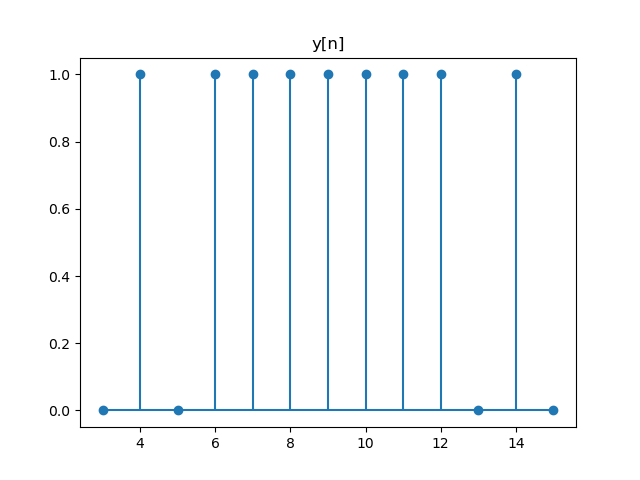
\includegraphics[width = .5\textwidth]{conv.png}
        \end{center}
        \item Is this system stable? Justify your answer.
        \begin{center}
            Yes, this system is stable because y[n]'s amplitude is a direct multiple of x[n]'s amplitude, therefore has bounded input bounded output.
        \end{center}
        \item Is this system casual? Justify your answer.
        \begin{center}
            Yes, This system is causal because it only depends on past and present times.
        \end{center}
    \end{enumerate}
\end{enumerate}
\end{document}
